\documentclass[10pt]{article}
\usepackage{geometry}
\geometry{a4paper,scale=0.8,includehead,includefoot}

\usepackage{iidef}
\usepackage{graphicx}
%\usepackage{amsfonts}
\usepackage{amsmath}
\usepackage{amssymb}
\usepackage{amsthm}
\usepackage{algorithm}
\usepackage{algorithmic}
\usepackage{bm}
\usepackage{hyperref}
\usepackage{footmisc}
\usepackage{xcolor}
\def\R{\mathbb{R}}
\def\P{\mathcal{P}}
\usepackage{mathtools}

\DeclarePairedDelimiter\abs{\lvert}{\rvert}
\DeclarePairedDelimiter\norm{\lVert}{\rVert}
\DeclarePairedDelimiter\inner{\langle}{\rangle}
\def\red#1{\textcolor{red}{#1}}
\theoremstyle{definition}
\newtheorem{definition}{Definition}
\newtheorem{theorem}{Theorem}
\newtheorem{example}{Example}
\newtheorem{proposition}{Proposition}
\newtheorem{corollary}{Corollary}
\newtheorem{lemma}{Lemma}
\newtheorem{remark}{Remark}

\renewcommand{\baselinestretch}{1.5}






\usepackage{color} 
\usepackage{listings} 
\usepackage{setspace} 

\definecolor{Code}{rgb}{0,0,0} 
\definecolor{Decorators}{rgb}{0.5,0.5,0.5} 
\definecolor{Numbers}{rgb}{0.5,0,0} 
\definecolor{MatchingBrackets}{rgb}{0.25,0.5,0.5} 
\definecolor{Keywords}{rgb}{0,0,1} 
\definecolor{self}{rgb}{0,0,0} 
\definecolor{Strings}{rgb}{0,0.63,0} 
\definecolor{Comments}{rgb}{0,0.63,1} 
\definecolor{Backquotes}{rgb}{0,0,0} 
\definecolor{Classname}{rgb}{0,0,0} 
\definecolor{FunctionName}{rgb}{0,0,0} 
\definecolor{Operators}{rgb}{0,0,0} 
\definecolor{Background}{rgb}{0.98,0.98,0.98} 
 
\lstdefinelanguage{Python}{ 
numbers=left, 
numberstyle=\footnotesize, 
numbersep=1em, 
xleftmargin=1em, 
framextopmargin=2em, 
framexbottommargin=2em, 
showspaces=false, 
showtabs=false, 
showstringspaces=false, 
frame=l, 
tabsize=4, 
% Basic 
basicstyle=\ttfamily\small\setstretch{1}, 
backgroundcolor=\color{Background}, 
% Comments 
commentstyle=\color{Comments}\slshape, 
% Strings 
stringstyle=\color{Strings}, 
morecomment=[s][\color{Strings}]{"""}{"""}, 
morecomment=[s][\color{Strings}]{'''}{'''}, 
% keywords 
morekeywords={import,from,class,def,for,while,if,is,in,elif,else,not,and,or,print,break,continue,return,True,False,None,access,as,,del,except,exec,finally,global,import,lambda,pass,print,raise,try,assert}, 
keywordstyle={\color{Keywords}\bfseries}, 
% additional keywords 
morekeywords={[2]@invariant,pylab,numpy,np,scipy}, 
keywordstyle={[2]\color{Decorators}\slshape}, 
emph={self}, 
emphstyle={\color{self}\slshape}, 
% 
} 
\title{Learning From Data Review Session}
%\author{Weida Wang, Feng Zhao}
\date{Sept. 2020}


\thecourseinstitute{Tsinghua-Berkeley Shenzhen Institute}
\thecoursename{Learning From Data}
\hwname{Review Session}
\theterm{Fall 2020}
\begin{document}
\courseheader
\name{Weida Wang, Feng Zhao}
\rule{\textwidth}{2pt}
%\maketitle

Aim: This note is to review some basic mathematical knowledge on linear algebra, calculus and probability, and to introduce some scientific programming background in Python. We hope it can assist you in your future coursework.

\section{Linear Algebra}
\subsection{Inner Product and trace}

\begin{definition}(Inner product). A function $\left<\cdot,\cdot\right>$: $\mathbb{V} \times \mathbb{V} \rightarrow \mathbb{F}$ is an inner product if it satisfies \cite{Gilbert}:\\

$\bullet$ \textbf{Linearity}: $\left<\alpha \bm{v} + \beta \bm{w}, \bm{x}\right> = \alpha\left<\bm{v}, \bm{x}\right> + \beta\left<\bm{w},\bm{x}\right>$;\\

$\bullet$ \textbf{Conjugate symmetry}: $\left<\bm{v}, \bm{w}\right> = \overline{\left<\bm{w},\bm{v}\right>}$;\\

$\bullet$ \textbf{Positive definiteness}: $\left<\bm{v}, \bm{v}\right> \geq 0$, with the equality iff $\bm{v} = 0$;\\
\end{definition}

The main example is the canonical inner product on $\mathbb{R}^{n}$, which simply sets
\begin{align*}
\left<\bm{x}, \bm{y}\right> =x_1 y_1 + x_2 y_2 + \cdots x_n y_n = \sum_{i=1}^{n} x_i y_i.
\end{align*}
And we say vector $\bm{x}\in\mathbb{R}^n$ is orthogonal to $\bm{y}\in\mathbb{R}^n$ when $\left<\bm{x}, \bm{y}\right>=0$.\\
The $\mathbf{Q} \in \mathbb{R}^{n \times n}$ is said to be \textbf{orthogonal} if its columns are pairwise orthogonal, which implies that 
\begin{equation*}
\mathbf{Q}\mathbf{Q}^{\mathrm{T}} = \mathbf{Q}^{\mathrm{T}}\mathbf{Q} = I
\end{equation*}
\begin{definition}(Trace).
For $\mathbf{M} \in \mathbb{R}^{n\times n} , \mathrm{trace}(\mathbf{M}) = \sum\limits_{i=1}^n \mathbf{M}_{ii}$, where $\mathbf{M}_{ii}$ is the diagonal terms of matrix $\mathbf{M}$.
\end{definition}
\begin{theorem}
 For any matrices $\mathbf{A}, \mathbf{B}$ of compatible size,
 \begin{align*}
     \mathrm{trace}(\mathbf{A}\mathbf{B})=\mathrm{trace}(\mathbf{B}\mathbf{A})
 \end{align*}
\end{theorem}


\subsection{Eigenvalue Decomposition}
\begin{definition}
(Eigenvalue, eigenvector). Let $\bm{A}\in \mathbb{C}^{n\times n}.$ We sat that $\lambda \in \mathbb{C}$ is an eigenvalue of $\bm{A}$ if there exists some nonzero vector $\bm{v}\in \mathbb{C}^{n}\setminus \left\{\bm{0}\right\}$ such that
\begin{align*}
    \bm{A}\bm{v} = \lambda\bm{v}
\end{align*}
\end{definition}

\begin{theorem}
 (Eigenvector decomposition). Let $\bm{A}\in\mathbb{R}^{n\times n}$ be symmetric. Then there exist orthonormal vectors $\bm{v}_1,\dots,\bm{v}_n \in \mathbb{R}^n$ and real scalars $\lambda_1 \geq\dots\geq \lambda_n$, such that if we write
 \begin{align*}
     \bm{V} = \left[\bm{v}_1|\dots|\bm{v}_n\right]\in O(n), \quad
     \Lambda = \begin{bmatrix} \lambda_1&&&\\&\lambda_2&&\\&&\ddots&\\&&&\lambda_n \end{bmatrix}\in \mathbb{R}^{n\times n},
 \end{align*}
 we have
 \begin{align*}
     \bm{A} = \bm{V}\Lambda\bm{V}^{*}.
 \end{align*}
\end{theorem}
The expression $\bm{A} = \bm{V}\Lambda\bm{V}^{*}$ can also be written as $\bm{A}=\sum\limits_{i=1}^{n}\lambda_i \bm{v}_i \bm{v}_i^*$.

\subsection{Vector and Matrix Norms}
A norm on a vector space $\mathbb{V}$ gives a way of measuring lengths of vectors. Formally:
\begin{definition}(Vector norm).
A norm on a real vector space $\mathbb{V}$ is a function $||\cdot||: \mathbb{V} \rightarrow \mathbb{R}$ that is:\\
$\bullet$ \textbf{Nonnegatively homogeneous}: $||\alpha \bm{x}||=\abs{\alpha}||\bm{x}||$ for all vectors $\bm{x}\in \mathbb{V}$, scalars $\alpha \in \mathbb{R}$;\\
$\bullet$ \textbf{Positive definite}: $||\bm{x}||\geq 0$, and $||\bm{x}|| =0$ iff $\bm{x}=0$;\\
$\bullet$ \textbf{Subadditive}: $||\cdot||$ satisfies the triangle inequality $||\bm{x} + \bm{y}|| \leq ||\bm{x}|| + ||\bm{y}||$, for all $\bm{x}, \bm{y} \in \mathbb{V}$.
\end{definition}

One very important family of norms are the $\mathcal{\ell}^p$ norms. If we take $\mathbb{V}=\mathbb{R}^n$, and $p\in [1,\infty)$, we can write
\begin{align}\label{eq.def}
||\bm{x}||_p = \left(\sum_i |\bm{x}_i|^p\right)^{\frac{1}{p}}.
\end{align}

The most familiar example is the $\ell^2$ norm or the "Euclidean norm"
\begin{align*}
    ||\bm{x}||_2 = \sqrt{\sum_i \bm{x}_i^2} = 
    \sqrt{\bm{x}^{\mathrm{T}}\bm{x}}
\end{align*}
which coincides with our usually way of measuring lengths. Two other cases are of almost equal importance: $p =1$, and $p\rightarrow \infty$. Setting $p=1$ in (\ref{eq.def}), we obtain

\begin{align*}
    ||\bm{x}||_1 = \sum_i |\bm{x}_i| .
\end{align*}

Finally, as $p$ becomes larger, the expression in (\ref{eq.def}) accentuates large $|\bm{x}_i|$. As $p\rightarrow \infty$, $||\bm{x}||_p \rightarrow \max_{i}|\bm{x}_i|$. Thus, we can extend the definition of the $\ell^p$ norm to $p=\infty$ by defining
\begin{align*}
    ||\bm{x}||_\infty = \max_i |\bm{x}_i| .
\end{align*}

Likewise, we can give the norm of matrices which characterizes the feature of matrices. \\
\begin{definition}(Matrix norm).
A norm on a real matrix space $\mathbb{R}^{m\times n}$ is a function $||\cdot||: \mathbb{R}^{m\times n} \rightarrow \mathbb{R}$ that is:\\
$\bullet$ \textbf{Nonnegatively homogeneous}: $||\alpha \bm{A}||=\abs{\alpha}||\bm{A}||$ for all matrices $\bm{A}\in \mathbb{R}^{m\times n}$, scalars $\alpha \in \mathbb{R}$;\\
$\bullet$ \textbf{Positive definite}: $||\bm{A}||\geq 0$, and $||\bm{A}|| =0$ iff $\bm{A}=\bm{0}$;\\
$\bullet$ \textbf{Subadditive}: $||\cdot||$ satisfies the triangle inequality $||\bm{A} + \bm{B}|| \leq ||\bm{A}|| + ||\bm{B}||$, for all $\bm{A}, \bm{B} \in \mathbb{R}^{m\times n}$;\\
$\bullet$ \textbf{Submultiplicativity}:  $||\bm{A}^{\mathrm{T}} \bm{B}|| \leq ||\bm{A}||||\bm{B}||$.

\end{definition}

The most famous matrix norms are Frobenius norm and spectral norm which are given by
\begin{align*}
    &||\bm{A}||_F = \left(\sum_{i=1}^{m}\sum_{j=1}^{n} a_{ij}^2\right)^{\frac{1}{2}}=\left(\mathrm{trace}(\bm{A}^{\mathrm{T}}\bm{A})\right)^{\frac{1}{2}}=\left(\sum_{i=1}^{m\bigwedge n} \lambda_i\right)^{\frac{1}{2}}\\
    &||\bm{A}||_s = \sqrt{\lambda_{max}},
\end{align*}
in which $\lambda_{max}$ is the largest eigenvalue of $\bm{A}^{\mathrm{T}}\bm{A}$.


\section{Calculus}
\subsection{Derivatives}
For scalar $b$,  vectors $\bm{x}, \bm{w}, \bm{y}$ and matrix $\bm{A}$, we have \cite{matrixcook}:\\
$\bullet$ $\dfrac{\partial(\bm{w}^{\mathrm{T}}\bm{x} + b)}{\partial\bm{x}} = \bm{w}$\\
$\bullet$ $\dfrac{\partial(\bm{x}^{\mathrm{T}}\bm{A}\bm{x} + b)}{\partial\bm{x}} = \bm{A}\bm{x}+\bm{A}^{\mathrm{T}}\bm{x}$\\
$\bullet$ $\dfrac{\partial (\bm{x}^{\mathrm{T}}\bm{A}^{-1}\bm{y})}{\partial\bm{A}} = -\bm{A}^{-\mathrm{T}}\bm{x}\bm{y}^{\mathrm{T}}\bm{A}^{-\mathrm{T}}$



\section{Probability}
\subsection{Basic Properties}

For events $E_1$ and $E_2$, if they are disjoint, i.e. $E_1 \cap E_2 = \emptyset$, then $\mathbb{P}(E_1 \cup E_2) = \mathbb{P}(E_1) + \mathbb{P}(E_2)$\\
\begin{definition}(Conditional probability) For events $A$ and $B$, and $\mathbb{P}(A)>0$,
\begin{align*}
    \mathbb{P}(B|A) = \frac{\mathbb{P}(A \cap B)}{\mathbb{P}(A)}
\end{align*}
	We can define the conditional expectation as 
	\begin{equation*}
	\mathbb{E}\left[Y|X=x\right] \triangleq\ \sum_{y\in \mathcal{Y}}y \cdot p\left(Y=y|X=x\right)
	\end{equation*}
\end{definition}
For two random variables $X$ and $Y$, the covariance is defined by
	\begin{equation*}
	\mathrm{Cov}\left[X,Y\right]=\mathbb{E}\left[XY\right]-\mathbb{E}\left[X\right]\mathbb{E}\left[Y\right]
	\end{equation*}
	When the covariance of $X$ and $Y$ is $0$, we call them uncorrelated variables.\\
	For two random variables, when the joint pdf can be written as the product of two RVs' pdf
	\begin{equation*}
	f\left(x,y\right)=f_X\left(x\right)f_Y\left(y\right),
	\end{equation*} 
	we call them independent.\\
\begin{theorem} We have:\\
$\circ$ (Multiplication Rule) For events $A$ and $B$,
\begin{align*}
\mathbb{P}(A \cap B) = \mathbb{P}(A)\mathbb{P}(B|A) = \mathbb{P}(B)\mathbb{P}(A|B);
\end{align*}
$\circ$ (Total probability rule) $B_1,B_2,\dots,B_k$ form a partition of $\Omega$, $\forall i \neq j, B_i\cap B_j = \emptyset, \cup^{k}_{i = 1} B_i = \Omega$, we have:
\begin{align*}
\mathbb{P}(A) = \sum_{i=1}^{k} \mathbb{P}(B_i)\mathbb{P}(A|B_i);
\end{align*}
$\circ$ (Bayes Rule)
\begin{align*}
\mathbb{P}(B_1|A) = \frac{\mathbb{P}(A \cap B_1)}{\mathbb{P}(A)}=\frac{\mathbb{P}(A | B_1)\mathbb{P}(B_1)}{\mathbb{P}(A)} = \frac{\mathbb{P}(A | B_1)\mathbb{P}(B_1)}{\sum\limits_{i=1}^k \mathbb{P}(A | B_i)\mathbb{P}(B_i)}.
\end{align*}
\end{theorem}


\subsection{Gaussian Distribution}
\subsubsection{Normal Distribution}
$\bullet$ If random variable $ X \in \mathbb{R}$, $ X\sim \mathcal{N}(\mu,\sigma^2)$, then the density function of it is:
\begin{align*}
    p(x;\mu,\sigma) = \frac{1}{\sqrt{2\pi\sigma^2}}e^{-\frac{1}{2} \left(\frac{x-\mu}{\sigma}\right)^2}
\end{align*}
$\bullet$ $\mathbb{E}[X] = \mu$; var$(X) = \sigma^2$.

\subsubsection{Multivariate Gaussian Distribution}
$\bullet$ If random variable $\bm{X}\in \mathbb{R}^{n}$, $ \bm{X}\sim \mathcal{N}(\bm{\mu},\bm{\Sigma})$, then the density function of it is:
\begin{align*}
    p(\bm{x};\bm{\mu},\bm{\Sigma}) = \frac{1}{(2\pi)^{n/2}|\bm{\Sigma}|^{1/2}}\exp{\left(-\frac{1}{2}(\bm{x}-\bm{\mu})^{\mathrm{T}}\bm{\Sigma}^{-1}(\bm{x}-\bm{\mu})\right)}
\end{align*}

$\bullet$ $\mathbb{E}[\bm{X}] = \bm{\mu}$; cov$(\bm{X}) = \bm{\Sigma}$.

\begin{figure}[htp]
\centering
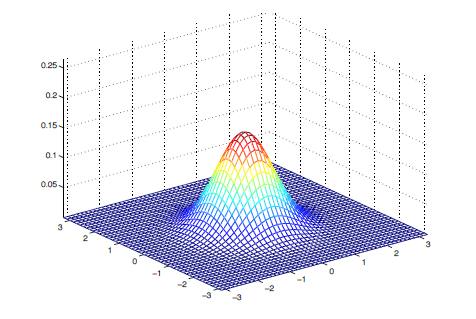
\includegraphics[width=0.75\linewidth]{multigaussian.png}
\caption{Multivariate Gaussian's p.d.f}
\end{figure}












\section{Scientific Programming in Python}
Python is a general purpose programming language.
With the help of some powerful packages, it is
possible to do scientific computing with Python.
In this section, a short introduction on how to
do scientific programming is given. To be more
specific, we will introduce how to use \texttt{numpy},
\texttt{scipy} and \texttt{matplotlib} to do linear algebra, statistics and basic 2D plotting.
\subsection{Numpy -- n-dimensional array manipulation}
The package \texttt{numpy} provides a convenient way for operations on n-dimensional array. As a special case, the vector is 1-dimensional array while the matrix is called 2-dimensional array. These two structures are the most commonly
used in practice. The following code shows how to create a vector of length 3 and compute its $\ell_2$ norm.
\begin{lstlisting}[language=Python]
import numpy as np
a = np.array([1, 2, 3])
print(np.linalg.norm(a))
\end{lstlisting}
As is noticed, most methods related with linear algebra are
under the module prefix \texttt{np.linalg}. We give another example to compute the eigenvalues of a square matrix:
\begin{lstlisting}[language=Python,firstnumber=4]
A = np.array([[1, 2], [3, 4]])
print(np.linalg.eig(A)[0])
\end{lstlisting}
The function \texttt{np.linalg.eig} returns two values,
the first is the eigenvalues and the second is the eigenvectors. Therefore, we use the index \texttt{[0]} to retrieve
only the first return value in the above code.
For detailed documentation, you can use \texttt{help(np.linalg.eig)}.
There are some advanced techniques to manipulate two-dimensional array. For example, if we want to compute
the summation of each row for a matrix. we can provide an
optional parameter \texttt{axis=1} as follows:
\begin{lstlisting}[language=Python, firstnumber=6]
A = np.array([[1, 2], [3, 4], [5, 6]])
print(np.sum(A, axis=1))
\end{lstlisting}
Notice that \texttt{A} is a $3 \times 2$ matrix. After the
operation of the \textbf{reduced sum} on \texttt{A}, we get a vector.
Another way to add together each row of
a matrix is to use matrix product.
Contrary to the mathematical representation, in \texttt{numpy},
\texttt{A * B} is the element-wise multiplication while \texttt{A @ B} is the
matrix product. Therefore, we need the
following code to achieve our goal:
\begin{lstlisting}[language=Python,firstnumber=8]
print(A @ np.array([1, 1]))
\end{lstlisting}
\subsection{Scipy -- algorithms of applied mathematics}
The package \texttt{scipy} provides many useful algorithms on various domains. In this subsection, we focus on the subpackage \texttt{scipy.stats}.

You have already known that a continuous random variable has
its probability density function (pdf). Theses functions are available in \texttt{scipy.stats}. For example,
the pdf of normal distribution can be queried by:
\begin{lstlisting}[language=Python,firstnumber=9]
import scipy.stats
x = np.linspace(-3, 3)
y = scipy.stats.norm.pdf(x)
print(x, y)
\end{lstlisting}
In this code snippet, we have used the function \texttt{np.linspace} to generate a vector of length 50.
As the function name suggests, the distances between adjacent numbers are equal. Then we apply the function \texttt{scipy.stats.norm.pdf} to this vector. It should be
noticed that \texttt{numpy} and \texttt{scipy} functions can
be applied to array directly. In logic, it is equivalent to apply
each element of the array and combine the result to an array.
But it is much faster to use array as the input parameter instead of writing a for-loop by hand.
\subsection{Matplotlib -- plotting experiment results}
The package \texttt{matplotlib} provides drawing method to
plot figures from data. We illustrate the basic usage of this
package by considering a simple experiment. That is,
we sample data from a Gaussian distribution, get the
empirical distribution by drawing the histogram and compare
the histogram with the Gaussian pdf. The code for this
procedure is as follows:
\begin{lstlisting}[language=Python,firstnumber=13]
import matplotlib.pyplot as plt
c = np.random.normal(size=1000)
plt.hist(c, density=True)
plt.plot(x, y)
plt.show()
\end{lstlisting}
We use the function \texttt{np.random.normal}
to generate 1000 random samples, which are used to draw the density histogram by \texttt{plt.hist}. We also
draw the true pdf by \texttt{plt.plot}. This plot function can accept two vectors and plot
a line on 2D plane. Finally, we use \texttt{plt.show} to open the figure window and we can see the plotting results immediately.
\subsection{Summary}
The above paragraphs only give a basic overview on the scientific packages of Python.
They are building-blocks of many machine-learning packages.
If you would like to learn more on this topic, I recommend a
good web resource written by Justin Johnson \cite{numpy}.

\begin{thebibliography}{9}
\bibitem{Gilbert} Strang, Gilbert, et al. Introduction to linear algebra. Vol. 3. Wellesley, MA: Wellesley-Cambridge Press, 1993.
\bibitem{matrixcook} The Matrix Cookbook  http://matrixcookbook.com 
\bibitem{numpy} https://cs231n.github.io/python-numpy-tutorial/

\end{thebibliography}
\end{document}
